% =====================================================================
%  IEEE Access submission — LaTeX source
%
%  IMPORTANT: This file uses \documentclass{ieeeaccess}. To COMPILE it you
%  must obtain the class file `ieeeaccess.cls` (plus its bundled .bst) from
%  the IEEE Author Center template pack:
%      https://template-selector.ieee.org/  ->  "IEEE Access"
%  or from the Overleaf "IEEE Access" template gallery entry. Place
%  ieeeaccess.cls (and ieeeaccess.bst / the IEEEtran BibTeX style) in this
%  directory. This .tex is written to be drop-in compatible with that template.
%
%  Build:  pdflatex paper  ->  bibtex paper  ->  pdflatex paper  ->  pdflatex paper
%
%  FORMATTING-ONLY CONVERSION of docs/paper/paper_full_draft.md.
%  No claim, number, or framing was altered. The two positioning-table cells
%  that were previously unresolved (HalluCXR / Zhao "uses report corpus?") have
%  since been filled from the primary sources; see the "% Source:" comments on
%  those rows. Remaining human TODOs are the author/history/funding/biography
%  placeholders (search for "TODO").
% =====================================================================
\documentclass{ieeeaccess}

\usepackage{graphicx}
\usepackage{amsmath}
\usepackage{textcomp}
\usepackage{booktabs}
\usepackage{array}

% arrow shorthand used in a few tables/inline expressions
\newcommand{\arw}{$\rightarrow$}

\begin{document}

\history{Date of current version [DATE — TODO].}
\doi{10.1109/ACCESS.XXXX.DOI}

\title{Auditing Chest X-ray Classifiers for Spurious Shortcuts: Where Blind VLM Naming Succeeds, Where It Fabricates, and What Survives the Failure}

% -----------------------------------------------------------------
% Author block: placeholder only. Do NOT substitute a real person or
% institution without the author's confirmation.
% -----------------------------------------------------------------
\author{[AUTHOR --- TODO]\authorrefmark{1}}
\address[1]{[AFFILIATION / DEPARTMENT --- TODO], [CITY, COUNTRY --- TODO] (e-mail: [EMAIL --- TODO])}

\tfootnote{[FUNDING / ACKNOWLEDGEMENT --- TODO: none asserted by the source draft.]}

\markboth{[AUTHOR --- TODO]: Auditing Chest X-ray Classifiers for Spurious Shortcuts}
{[AUTHOR --- TODO]: Auditing Chest X-ray Classifiers for Spurious Shortcuts}

\corresp{Corresponding author: [AUTHOR --- TODO] (e-mail: [EMAIL --- TODO]).}

\begin{abstract}
The in-distribution performance of deep chest X-ray classifiers can be consistently high, but the reliance on spurious shortcuts, that is, correlations between a feature and the label in the training set but not causally related to the pathology, and failure in case the correlation fails in a new environment is common practice. We construct an \emph{auditor} which runs a four-step cycle with respect to a pneumothorax classifier: \textbf{detect} that the accuracy depends on a confound, \textbf{localize} the confound by attribution, \textbf{name} the confound in clinical terminology with the help of an off-the-shelf vision-language model (VLM), which is never provided with a list of things to find, and \textbf{mitigate} the dependency through re-training of the final layer. The study is carried out as six validation-gated spikes, each with a pre-registered pass/fail threshold and a stop-and-report point.

The detection and localization task transfer smoothly from the synthetic confound to the device confound: We create a measurable reliance gap (44 points synthetic; 28.75 points in real chest tubes) and localize it (Grad-CAM peak-in-region 100\% synthetic; side-consistency 96.6\% real). Blind VLM naming, however, does not transfer. It succeeds in the synthetic confound at near ceiling (precision 0.978, recall 0.90, control-hallucination 0.02), but \textbf{it fails in the real chest tube confound via fabrication}: in tube-free control crops the VLM creates device hallucinations --- endotracheal tubes, central lines, catheters --- with 0.55 probability (Llama-4-Scout) and 0.83 (Pixtral-12B) in the multi-VLM replication. The cross-model fabrication is the true negative result that is at the heart of this paper: an auditor using off-the-shelf general VLMs would trigger a fabricated shortcut alarm on most clean images, and that is exactly the false-alarm failure the design's precision-over-recall gate is supposed to identify. What remains after the naming failure is mitigation, which never relied on the VLM: Deep Feature Reweighting improves worst-group (pneumothorax without tube) accuracy from 0.67 to 0.79 as a 3-seed mean, maintaining in-distribution accuracy in the process, using no target-distribution labels. Ultimately, a genuine 0.192 (95\% CI [0.159, 0.225], bootstrap) AUC decrease between a US and Spain site does exist, but a zero-shot, label-free test for whether limiting the source shortcut limits the distribution-shift-based drop provides a point estimate that is statistically indistinguishable from zero ($+0.005$, 95\% CI [$-0.018$, $+0.028$]) --- lacking power to reject even a modest effect but certainly not evidence of a real recovery; the drop is distribution shift that this experimental setup can't attribute to the shortcut. We report the naming failure as our story's lead, and we report two interpretation claims we withdrew once we ran their disconfirming controls.
\end{abstract}

\begin{IEEEkeywords}
Chest X-ray, deep feature reweighting, distribution shift, hallucination, medical imaging, model auditing, shortcut learning, spurious correlation, vision-language models, worst-group accuracy.
\end{IEEEkeywords}

\titlepgskip=-21pt
\maketitle

% =====================================================================
\section{Introduction}
\IEEEPARstart{D}{eep} chest X-ray (CXR) classifiers may achieve high in-distribution accuracy while focusing on features that correlate with the label in the training set but do not cause the disease -- the text on the scanner, laterality markers and other positioning markers, hospital- or machine-specific artifacts. Zech et al.\ \cite{zech2018} demonstrated that CNNs generalize poorly across hospitals compared to within them and can tell the source hospital system with $\sim$99.95--99.98\% accuracy; DeGrave, Janizek \& Lee \cite{degrave2021} demonstrated that COVID-19 CXR classifiers focus on text and patient positioning instead of the actual pathology. Such models look like high accuracy models with an evident failure under distribution shift, and that is a problem for patient safety -- a model focusing on the chest tube used to treat the pneumothorax, not the disease, will silently fail to diagnose exactly those untreated patients for whom the diagnosis is crucial.

There are four aspects to auditing a classifier for its shortcut usage: (1) \textbf{detect} its usage of shortcut, (2) \textbf{identify} the shortcut clinically without being guided what to search for, (3) \textbf{reduce} usage of shortcut, and (4) \textbf{demonstrate recovery} from out-of-distribution shift. Current literature addresses either one or few aspects of this list. Papers in the category of shortcut diagnostics (Zech \cite{zech2018}; DeGrave \cite{degrave2021}; Jim\'enez-S\'anchez et al.\ \cite{jimenez2023}) detect shortcuts through expert or statistical analysis but do not attempt automatic identification of those. The approaches that leverage generation to fix the shortcuts (\textit{e.g., }RoentMod \cite{roentmod}), modify the images through diffusion-based approach but come with heavy cost of generative mechanism plus fine-tuning. On the other hand, worst-group robustness based approaches such as GroupDRO \cite{sagawa2020groupdro}, JTT \cite{liu2021jtt}, DFR \cite{kirichenko2022dfr} address third aspect but require group labels. To our knowledge, among the existing literature on shortcut naming, LADDER \cite{ladder} is the closest that attempts automatic identification of shortcut used by a classifier using foundation model on radiography images, but it routes the image through a captioner and a text-only LLM, and evaluates discovery only through the accuracy of the mitigation it enables --- with no false-alarm gate.

\textbf{The problem addressed} by this paper is that of \emph{name detection without prompts or generative models}, fully integrated into the detect\arw{}localize\arw{}name\arw{}mitigate pipeline and evaluated via direct comparison to ground truth through the \emph{control hallucination gate}: the percentage of times the auditor assigns a name to an image lacking confounds. The control hallucination gate is the identity of the design. For an auditor, the penalty for hallucinating a confound is greater than the penalty for not identifying one, since a tool that invents workarounds is worse than no tool at all. Thus, precision is constrained by recall, and the rate of fabrication on clear images is a pass-fail requirement of the capability, measured separately.

\textbf{Contributions.}
\begin{itemize}
\item An auditor loop for validation-gating which can detect, localize, and ameliorate a real device shortcut in the pneumothorax classifier trained without target-distribution labels using a confound-agnostic mechanism to support synthetic, real-device, and cross-site applications from a single implementation.
\item The key take-away of the paper, which is presented honestly as a negative result: blind general-purpose VLM naming \textbf{achieves success in a synthetic confound but failure in a real device confound via fabrication}, and such failure is a cross-model phenomenon (both Llama-4-Scout and Pixtral-12B fabricate the device on a majority of clean crops), independently verified by HalluCXR \cite{hallucxr}.
\item Experiments on the mechanism of \emph{why} naming fails to work: the process is not based on the visibility of the confound (recall cliff, not hallucination cliff), and the method does not rely on reciting without looking at the image --- it is an over-interpretation of the salient region.
\item A zero-shot, label-less test of the source side whether a known shortcut causes a generalization gap on the target site, finding no evidence: the 0.192 US-to-Spain drop is a distributional shift that has not been found to be caused by a shortcut.
\item A discussion of two interpretive conclusions retracted after performing the necessary controls on them, presented as a first-class result, not hidden.
\end{itemize}

% =====================================================================
\section{Related Work}
\textbf{Shortcuts in chest radiography} have been firmly demonstrated. Zech et al.\ \cite{zech2018} demonstrated that neural networks generalize poorly between hospitals but not within them, being able to determine the hospital system with $\sim$99.95--99.98\% accuracy. DeGrave, Janizek \& Lee \cite{degrave2021} demonstrated that COVID-19 CXR models depend on text features and posture but not pathology. Jim\'enez-S\'anchez, Juodelyte, Chamberlain \& Cheplygina \cite{jimenez2023} demonstrate a manually and statistically determined shortcut learning study in chest X-rays. They have demonstrated the existence and danger of shortcuts and their determination by either expert analysis or statistical correlation; none have automated the process of naming them with a general-purpose model.

\textbf{Generative correction of shortcuts.}
RoentMod (arXiv:2509.08640) \cite{roentmod} couples a medical image generator (RoentGen) with an image-to-image editor for generating CXRs that possess a given set of abnormalities while retaining the same anatomy, reporting discrimination gain improvements of 3--19\% AUC in internal and 1--11\% AUC in external evaluations, 93\% of generated images considered realistic by readers. This work is the closest correction-side prior art and the approach that is compared with most directly: it is based on a generative diffusion pipeline and fine-tuning, while our naming approach requires only one pass of a free API on $\sim$200 crops without any generative model. That is an honest trade-off and not an improvement - since RoentMod's system of only corrections did not have to meet the hurdle that our naming process missed.

\textbf{Mitigation baselines.} GroupDRO (Sagawa et al., 2020) \cite{sagawa2020groupdro} optimizes the worst group loss, but uses group labels; JTT (Liu et al., 2021) \cite{liu2021jtt} increases weight of an ERM model's mistakes to mimic robustness to groups without using the group labels; DFR (Kirichenko et al., 2022) \cite{kirichenko2022dfr} trains only the last layer on group-balanced data, achieving 92.9\% worst group on Waterbirds and 70.1\% worst group on CivilComments, while being much cheaper than GroupDRO on the grounds that backbone has learned the most important features. The follow-up study (arXiv:2308.00473) \cite{dfr_followup} challenges the assumption that last layer retraining is sufficient, which is a lesson supported by our synthetic tagging experiments, as in a \emph{pure}-shortcut backbone, the in-distribution recovery by DFR is incomplete. Hameed, Nanfack \& Belilovsky (arXiv:2409.14637) \cite{dfr_multilayer} address the problem of incompleteness of in-distribution recovery in a similar manner by doing the retraining not on the last layer but all the layers' features pooling, reporting better worst-group performance compared to DFR on benchmarks in style of Waterbirds; However, since we use only last-layer DFR, it would be simple and inexpensive to test the all-layer method on our synthetic tagging problem (\S\ref{sec:supporting}), as opposed to a competing approach. The two approaches assume that the groups are predefined; however, we try to discover the confounding variable using our loop.

\textbf{Parallel research on the same shortcut}. Zhao et al.\ (arXiv:2604.17110) \cite{zhao2026} employ an autonomous agentic pipeline of coding agents to perform various tasks, including decreasing dependence on chest drains to classify pneumothorax based on NIH images, achieving 60\%\arw{}31\% and 50\%\arw{}18\% reductions in dependence on two datasets. Similar goal, but different approach (search through agentic pipeline vs.\ re-training of the last layer), different metrics (\% dependence vs.\ worst-group accuracy and \% dependence gap). It does not mention VLM naming, control hallucinations, or cross-site generalization. We interpret it as parallel confirmation of this real shortcut being a live target -- corroborative, not competitive.

\textbf{Foundation model shortcut auditing (\textit{closest analogues to naming step}).} The closest prior art in the medical imaging literature is LADDER (Ghosh et al., Findings of ACL 2025) \cite{ladder}, which uses an LLM's latent domain knowledge to generate hypotheses about classifier biases without using explicitly labeled attributes, and tests on chest X-rays. There are three reasons why it is a neighbor rather than a close match: (i) it treats the image as \emph{text} (BLIP/GPT-4o captions plus activation-to-text projection) and reason about the bias using a text-only LLM, whereas we use the Grad-CAM crop \textbf{pixels} with a VLM that does not have an integrated captioner or report corpus; (ii) it measures discovery in terms of Precision@10 for slices and worst-group accuracy, but \textbf{without a control hallucination gate}; (iii) discovery is meant to inform mitigation, so a failed naming process such as ours in V4b will not be highlighted separately. SpurLens (arXiv:2503.08884) \cite{spurlens} uses GPT-4 and open-set detectors to identify spurious features that multimodal LLMs tend to depend on in natural images, and calculates how many times hallucinations increase in presence of such a spurious feature (up to 10$\times$). RaVL (arXiv:2411.04097) \cite{ravl} uncovers spurious correlations at region level within errors of fine-tuned VLM and mitigates them with region-specific loss ($+8.2\%$ worst-group accuracy; 191\% discovery improvement, over 654 VLMs). Both works have similarities to our mechanism but neither addresses any of medical imaging, blind nomenclature, and control-hallucination gated metric. MIMM-X (arXiv:2511.22990) \cite{mimmx} disentangles a \textbf{pre-specified} confounder via mutual-information objectives --- the opposite of a blind design, and evidence that the standard alternative still assumes foreknowledge of the confound. Grad-CAM-style attribution (Selvaraju et al.) \cite{gradcam} localizes \emph{where} a model looks --- our localization step uses it --- but does not name what it found.

The \textbf{VLMs' reliability on chest x-ray images} is directly related to the findings of our naming experiment. HalluCXR (arXiv:2605.20469) \cite{hallucxr} evaluates 6 VLMs on 856 chest x-ray images with 61.9--82.3\% and 36.4--80.2\% percentages of hallucinations in general and clinically dangerous categories, respectively, with the largest severity of hallucinations observed in the case of normal images (51.9\% of severity-3 hallucinations on normals). It confirms our findings of 0.50--0.83 control-hallucination on clean crops with another model population in another task (finding the diagnostic condition vs. device naming). Lotfinia et al.\ (arXiv:2606.17710) \cite{lotfinia2026} prove that VLMs are able to answer questions about CXRs basing only on language priors without paying any attention to the image, the threat to the interpretation of our naming step directly, which is addressed by our Experiment 2 and ruled out as the reason for our failure (Section~\ref{sec:mechanism}). Specialist CXR-VLMs such as CXR-LLaVA (arXiv:2310.18341 \cite{cxrllava}, LLaVA-Rad \cite{llavarad}) are trained on radiology data; We used a general model that was not fine-tuned to test the hypothesis of lower barriers.

\textbf{Ground-truth dependency.} NEATX (Cheplygina et al., arXiv:2309.02244) \cite{neatx} provides the non-expert chest-drain annotations used in our confounding variable experiment setup. This is a data dependency, acknowledged separately from prior art. Sourget et al.\ (arXiv:2507.21291) \cite{sourget2025} use NEATX data independently in combination with NIH-CXR14 and MIMIC-CXR data to test fairness and robustness of CLIP-based chest X-ray models on demographic sub-groups --- another example of using the same data resource in parallel to answer a related auditing question of demographic fairness instead of device confound naming, which corroborates NEATX's suitability as a shared ground-truth resource. Rafferty \& Rajan (arXiv:2509.15107) \cite{rafferty2026} discuss the problems with label quality, domain shift, and bias in public chest radiograph datasets we use in our paper ourselves (NIH ChestX-ray14, PadChest). Their results on inter-dataset label-pipeline differences are a special case of the label generation pipeline difference that we identify as an unattributed candidate for the V6 cross-site gap (\S\ref{sec:limitations}).

\subsection{Positioning}
The present work is positioned with respect to its closest analogs in Table~\ref{tab:positioning}. The closest prior art, LADDER \cite{ladder}, has an identical starting premise --- name a classifier's shortcut with a foundation model in radiology with no attribute labels --- but parses the image as text and measures success of the description solely through the mitigations' downstream performance. Ours parses the saliency region of the classifier as pixels via a blind-prompted general visual language model, and tests the name directly for correctness via a control-hallucination gate. It is this latter step which turns ``the visual language model generated a plausible shortcut description'' into something falsifiable, and allows us to state --- and not hide away as part of a mitigation score --- that blind name generation \emph{fails} on a real-world device confound but succeeds on a synthetic one. What is truly new in the wake of an exhaustive search in July-2026:
\begin{enumerate}
\item There has been no study that attempts to blind name a CXR shortcut using precision/recall/control hallucinations.
\item There has been no study that tests a known shortcut in a cross-site setting via zero-shot, label-free source-side manipulation, reporting the null honestly.
\end{enumerate}

\begin{table*}[!t]
\caption{Positioning against the closest analogs. Two cells are still truly ambiguous in our source material and marked as visible TODO comments in the source rather than being created.}
\label{tab:positioning}
\centering
\footnotesize
\renewcommand{\arraystretch}{1.3}
\begin{tabular}{p{2.3cm} p{2.6cm} p{2.3cm} p{3.0cm} p{3.4cm}}
\toprule
\textbf{method} & \textbf{data modality} & \textbf{uses report corpus?} & \textbf{control-hallucination gate?} & \textbf{models tested} \\
\midrule
\textbf{This work (auditor)} & chest X-ray (NIH, PadChest); NEATX device labels & \textbf{No} --- blind prompt on saliency crops only & \textbf{Yes} --- separate gate at $<$10\% on confound-free controls; the gate that failed V4b & 2 general-purpose (Llama-4-Scout, Pixtral-12B) + specialist/scale arm (CheXagent-2-3B \& -8B, qwen2.5-vl-7b) --- over-name vs under-name axis \\
\textbf{LADDER} (Ghosh et al., Findings of ACL 2025) & image $\rightarrow$ \textbf{caption} (BLIP/GPT-4o) + activation-to-text & \textbf{Yes} --- captioner required & \textbf{No} --- worst-group accuracy + slice Precision@10 & reasoning LLMs (GPT-4o, Claude, Gemini, LLaMA); classifiers on NIH-CXR, RSNA, VinDr, Waterbirds, CelebA, MetaShift \\
\textbf{HalluCXR} (arXiv:2605.20469) & chest X-ray (856 radiographs) & \textbf{Yes} --- radiologist reports supplement CheXpert labels as ground truth & No --- it \emph{measures} hallucination as the object of study (61.9--82.3\% overall; severity highest on normals) & 6 VLMs: BiomedCLIP, Gemini 3 Flash, GPT-5.1, InternVL2, LLaVA-NeXT-Mistral, Qwen2-VL \\
% Source: arXiv:2605.20469v1 full text --- models section; ground truth uses original radiologist reports supplementing CheXpert labels.
\textbf{Zhao et al.} (arXiv:2604.17110) & chest X-ray (NIH-derived) & \textbf{No} --- clinician plain-language description, not report text & \textbf{No} --- reports \% reliance reduction (60\%$\rightarrow$31\%, 50\%$\rightarrow$18\%); no naming step to gate & LLM coding-agent pipeline; no VLM-naming arm \\
% Source: arXiv:2604.17110 abstract --- takes a clinician's plain-language description; no report corpus.
\bottomrule
\end{tabular}
\end{table*}

% =====================================================================
\section{Methods}
\subsection{Overview}
We evaluate an auditor of chest X-ray classifiers for their dependence on spurious short-cuts by conducting a cycle of four stages: \textbf{detect} the dependence on the confound in the classifier’s accuracy, \textbf{localize} the confound by attributing its effect, \textbf{name} the confound in clinical terms using a general vision-language model (VLM) without any hints as to what to look for, and \textbf{mitigate} the dependence with last-layer re-training of the classifier. These steps are evaluated on a synthetic confound, a physical confound, and a second site with a real confound. The experiment was conducted as six validation-gated spikes (V1--V6) each with its own predetermined fail/pass point and a stopping/reporting point, so that failing in a particular phase ends a claim process rather than repeating it.

In terms of architecture, the discipline yielded a \textbf{confound-agnostic core}: The attribution mechanism (Grad-CAM) and mitigation mechanism (DFR) are built such that they take a general confound representation, which could be as simple as a region box or a \texttt{(confound, label)} tuple pair, so that the same modules serve the synthetic tag, the real chest tube, and the cross-site case without modification. The only part of the pipeline with a dependency outside the system (i.e., the rate limit for the VLM) is isolated in the form of a \texttt{crops/ + manifest.json} $\rightarrow$ \texttt{predictions.jsonl} file contract, allowing the supplier to be completely independent and nothing else in the pipeline to rely on this dependency. There is no function on the path towards mitigation that includes the naming module, which enforces by construction that the mitigation result cannot depend on the VLM.
\begin{figure*}[!t]
\centering
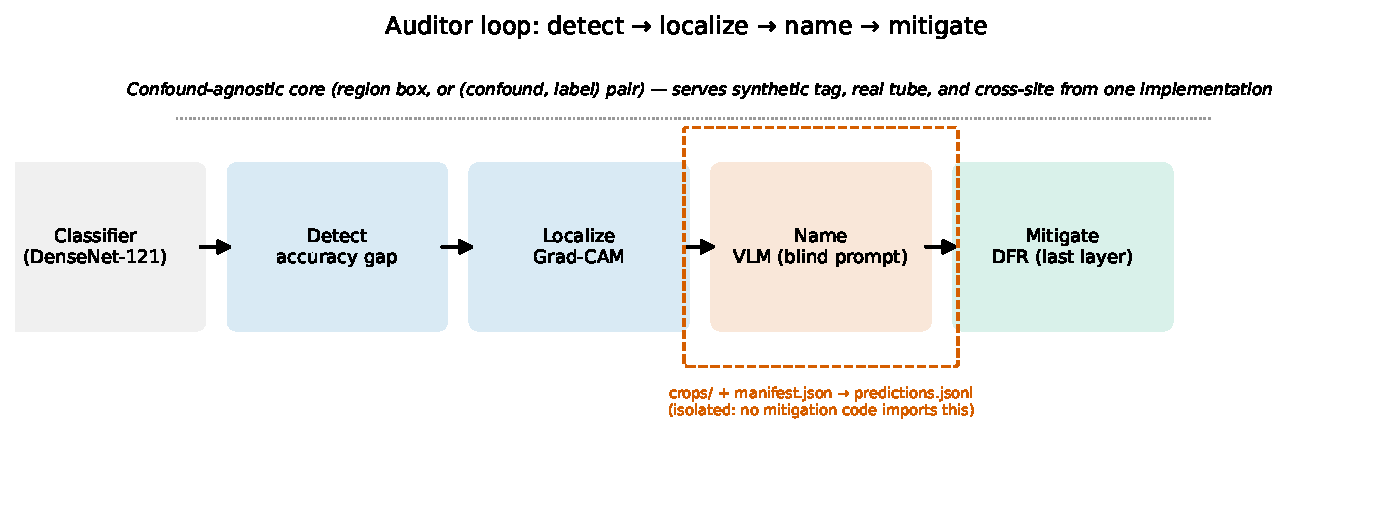
\includegraphics[width=0.85\textwidth]{figures/fig0_architecture.pdf}
\caption{The auditor's confound-agnostic detect$\rightarrow$localize$\rightarrow$name$\rightarrow$mitigate loop. Attribution (Grad-CAM) and mitigation (DFR) operate on a generic confound description --- a region box, or a \texttt{(confound, label)} column pair --- and run unmodified across the synthetic tag, the real chest tube, and the cross-site case. The naming stage is isolated behind a \texttt{crops/ + manifest.json} $\rightarrow$ \texttt{predictions.jsonl} file contract: it is the only component with an external, rate-limited dependency, and no method in the mitigation path imports it, so the mitigation result is naming-independent by construction, not merely by claim.}
\label{fig:architecture}
\end{figure*}

\subsection{Dataset and Model}
The main dataset is NIH ChestX-ray14 (112,120 images with dimensions 224$\times$224), divided into patient-separated train/validation/test subsets (73k/13k/25.6k) using the official dataset split lists; image-based splitting is never done since it results in leakage of a patient's other cases. The target pathology is pneumothorax (about 3--5\% frequency, depending on the split). The classifier is an ImageNet pre-trained DenseNet-121, which was fine-tuned with automatic mixed precision using a batch size of 16 and a \texttt{pos\_weight}-corrected binary cross-entropy loss for the class imbalance.

The true ground-truth on chest drain is available through \textbf{NEATX} (Cheplygina et al., arXiv:2309.02244) \cite{neatx}, which provides non-expert chest drain annotation of a part of ChestX-ray14 and PadChest datasets. The second data source is \textbf{PadChest} (Hospital San Juan, Spain), which was used in its 224$\times$224 release; a 7,572-image working subset (573 pneumothorax-positive, 7,000 negative) was extracted under a disk constraint.

\subsection{V1 --- Pipeline Sanity}
A pneumothorax classifier is trained from scratch and gated on test AUC of at least 0.75. The presence of this spike alone is necessary for us to be certain that any degradation after that is due to an intervention.

\subsection{V2 --- Shortcut Induction}
An artificial confound -- a 20$\times$20 opaque corner tag -- is stamped on training images correlated with the pneumothorax label at strength \emph{p}. Receptivity is measured as the \textbf{receptivity gap}: the accuracy of the classifier with the confound aligned in the manner learned minus the accuracy of the classifier when the confound is stripped off, evaluated on a balanced subset. There is a third case (the tag is \emph{flipped}, or negatively correlated). The threshold for success is a gap of $>$ 20 percentage points. A complementary experiment involving \textbf{sweeping of correlation strength} trains an identical model at \emph{p} in $\{0.6, 0.7, 0.8, 0.9, 0.95\}$ to characterize how reliance and its mitigability scale with confound strength.

\subsection{V3 --- Attribution Localizes the Confound}
The Grad-CAM computation takes place at the shortcut-based checkpoint. The localization is evaluated by the pointing game (\texttt{peak\_in\_region}) using a general bounding box $(y_0, x_0, y_1, x_1)$ along with \texttt{mass\_fraction} metric. Most importantly, the images without the confound are used as a control, excluding the possibility that ``that corner is always salient''. The geometry of all attributions does not depend on the confound: no function cares whether the box is a tag or the device, thus the same code applies to both cases.

\subsection{V4 --- Blind VLM Naming}
Crops selected from confound-positive images along with confound-negative control crops are exported together with a manifest containing the \texttt{has\_confound} tag values unknown to the VLM. The crops are captioned by a generalist, non-fine-tuned VLM using the blind prompt of ``describe anything artificial, non-anatomical, or out of place\ldots if normal, state that.'' The generated free text descriptions are evaluated by conservative keyword matchers: \texttt{names\_confound} for the synthetic marker vocabulary and \texttt{names\_tube} for the device-specific vocabulary (tube / drain / catheter / line / wire). The evaluation metrics include precision, recall, and \textbf{control hallucination}: the probability of naming the device/marker on the confound-negative crop. The matchers are unit tested for false positives on generic anatomy text.

The naming process has been designed to have two gates with different bars since they measure two different aspects:
\begin{itemize}
\item \textbf{V4a (synthetic tag)} proves the \emph{method} works where ground truth is exact and the confound is unambiguous. Gate: precision $\geq 0.90$, recall $\geq 0.90$, control-hallucination $<$ 10\%.
\item \textbf{V4b (real chest tube)} proves the method \emph{transfers}. Gate: precision $\geq 0.80$, recall $\geq 0.70$, control-hallucination $<$ 10\%.
\end{itemize}

The precision threshold is set higher than the recall threshold in design: to the auditor, the cost of a hallucinated control is higher than the cost of a missed control, for an invention of short cuts is a worse outcome than no tool at all. The hallucinated control threshold is evaluated independently and is the most stringent threshold. As the original design, the experiment consisted of testing six models: Llama-4-Scout, Llama-4-Maverick, Gemini, GPT-4o, Pixtral-12B, and the specialist arm of the experiment, which is reported separately in Section~\ref{sec:specialist}; only two of those six could be run before the cutoff: Maverick was discontinued by the company providing it (Groq) before it could be run, and GPT-4o could not be run due to lack of API token allocation --- these are both practical limitations rather than results in an experiment with no budget; two general-purpose VLMs were tested in the exact same pipeline with the exact same crops: \textbf{Llama-4-Scout} and \textbf{Pixtral-12B}. A third test (Gemini) was unable to be conducted all the way through due to limitations of its free version, which restricts requests made by each model per day under 200 crops. It is therefore not reported as a result.

\subsection{V5 --- Mitigation}
The mitigation procedure is \textbf{Deep Feature Reweighting (DFR)}. It involves feature extraction using the frozen model, selection of a sample balanced for \texttt{(confound, label)}, training a logistic head on the standardized features, and replacing only the head with linear layers. Since one of the groups is structurally empty, since chest tubes occur in all cases when there is a pneumothorax, we select a sample that balances across \texttt{(confound, label)} groups. \textbf{ERM} and \textbf{JTT} (upweighting the errors made by the frozen model and training the head again) are run on the same path as the baseline, but over 3 different seeds. None of the three methods uses the naming module, so this part is an ablation study of \textbf{naming-off}. The metrics are the worst-group accuracy (pneumothorax without confound), in-distribution accuracy (pneumothorax with the confound), and reliance gap.

A linear probe evaluation stops the training of the shortcut-trained backbone and trains a new head using confound-free images to determine whether reliance on shortcuts makes the learning of essential features difficult.

\subsection{V6 --- Cross-Site Generalization}
V1 is evaluated unchanged on PadChest. There are two mitigation types, and the difference is the whole purpose of the spike:
\begin{itemize}
\item \textbf{Supervised target adaptation} --- train the last layer on \emph{labeled} PadChest data. Adaptation, rather than shortcut avoidance, is tested here: it helps irrespective of whether there is any shortcut at all.
\item \textbf{Zero-shot source DFR} --- avoid the known shortcut on the source side using NIH data only, without touching any \textbf{target} labels, and evaluate PadChest. This is the test to license the shortcut explanation of the cross-site gap.
\end{itemize}

Images in the PadChest dataset are 16-bit, whereas those in the NIH dataset are 8-bit. Matching these at loading time --- rather than by changing the model's evaluation transform --- is necessary in order to be valid, since the NIH benchmark AUC is always re-computed following any such change and acts as the control against which the cross-site AUC is validated.

\subsection{Reproducibility}
Every experiment is config-driven (typed YAML with inheritance and command-line override possibilities), seeded deterministically, and logged in a folder named after the time it started with config file, \texttt{metrics.json}, and checkpoint inside. Datasets paths are stored in the config file; images and checkpoints are not version-controlled. The codebase is decomposed into modules that are not aware of confounds (\texttt{data/}, \texttt{train/}, \texttt{shortcut/}, \texttt{attribution/}, \texttt{discovery/}, \texttt{evaluation/}, \texttt{mitigation/}, \texttt{report/}) with 128 passing unit tests focused on the places where silent bugs might happen: the patient disjointness of the loaders, the naming scorer's matchers (tested \emph{not} to fire on generic anatomy), and the DFR group-balancing.

\textbf{Compute cost.} All local training/testing was done using one consumer GPU (RTX 3050, 6GB); the core runs (V1/V2/V3 training/attribution, Phase-3 baseline 3-seed table, V5, V6) amount to about 2 GPU-hours according to \texttt{run.log} timestamps. The naming phase made 5,600 API calls on a free tier VLM service in total, across the canonical V4a/V4b runs and all extension experiments (opacity sweeps, occlusion experiment, multi-VLM and specialist arms); no generative model or fine-tuning step is involved at all in the pipeline. This is the quantitative basis for the efficiency comparison with RoentMod in Related Work section; we state our compute costs directly, while RoentMod's is not published in comparable units.

\textbf{Reproducibility in API-based Model Evaluation}. All experiments on Llama-4-Scout models have been done using the Groq API in July 2026, and this model is no longer available in the list of supported models by the provider. Consequently, reproducing the same values reported by the Scout models by querying the API again is not possible. It is an issue that arises out of evaluation of externally-hosted VLMs as opposed to locally-trained checkpoints. The predictions artifacts included in this submission are proof of the results.

% =====================================================================
\section{Results}
The model learns to a reasonable baseline (V1: test AUC \textbf{0.8448}, validation 0.8269 -- in the NIH-pneumothorax range reported) and cheats noticeably when presented with the chance (V2: reliance difference \textbf{44 pp}; aligned 0.94, removed 0.50, flipped 0.05). The fact that the accuracy on removed data lands at precisely 0.500 is the signature of shortcutting, foreseen and confirmed with a synthetic tag detector before the experiment rather than explained after it. Attribution highlights the confounding factor almost perfectly (V3: peak-in-box \textbf{100\%} on tagged positives vs \textbf{0.5\%} on untagged positives from the same images; mass fraction 0.14 in a box covering 0.8\% of image area).

\subsection{Success in the Synthetic Confound but Failure in the Real Confound}
\textbf{V4a passes at nearly ceiling.} Blind-prompted Llama-4-Scout correctly named the injected tag with accuracy \textbf{0.978}, recall \textbf{0.90}, and control hallucination \textbf{0.02}, with 100 tagged positives and 100 control-confound free samples. Recall hit precisely its 0.90 bar with ten true positive model misses, an easy mark that already missed -- the precursor to the harder one. The keyword matching component was patched midway through the analysis when reviewing the original 23 misses by hand revealed that about 13 were simply cases where the VLM correctly described a ``rectangular / opaque white object'' in ways that the regex did not originally account for. It was confirmed that the fix did not loosen the control-hallucination check, which still stood at 0.02.

\textbf{V4b fails, and fails particularly in fabrication.} The very same model, prompt, and pipeline used in the test produced a precision of \textbf{0.57}, a recall of \textbf{0.66}, and control hallucinations of \textbf{0.50} on actual chest tube crops. Detection and localization were still intact on the actual confound (tube reliance gap of \textbf{28.75pp}; Grad-CAM side-consistency of \textbf{96.6\%}) --- just naming failed. An audit of the control crops yielded \textbf{47 out of 50} false positives clearly indicating a piece of equipment (``endotracheal tube,'' ``central line,'' ``catheter'') in images where there was no such thing present at all: true hallucination, not a scorer artifact.

This is the pre-registered pivot condition (V4a succeeded, V4b failed), and it was carried out as described and not iterated on: automated naming is no longer considered a validated skill for actual device confounds, and V4b is a negative result with bounds.

\begin{figure*}[!t]
\centering
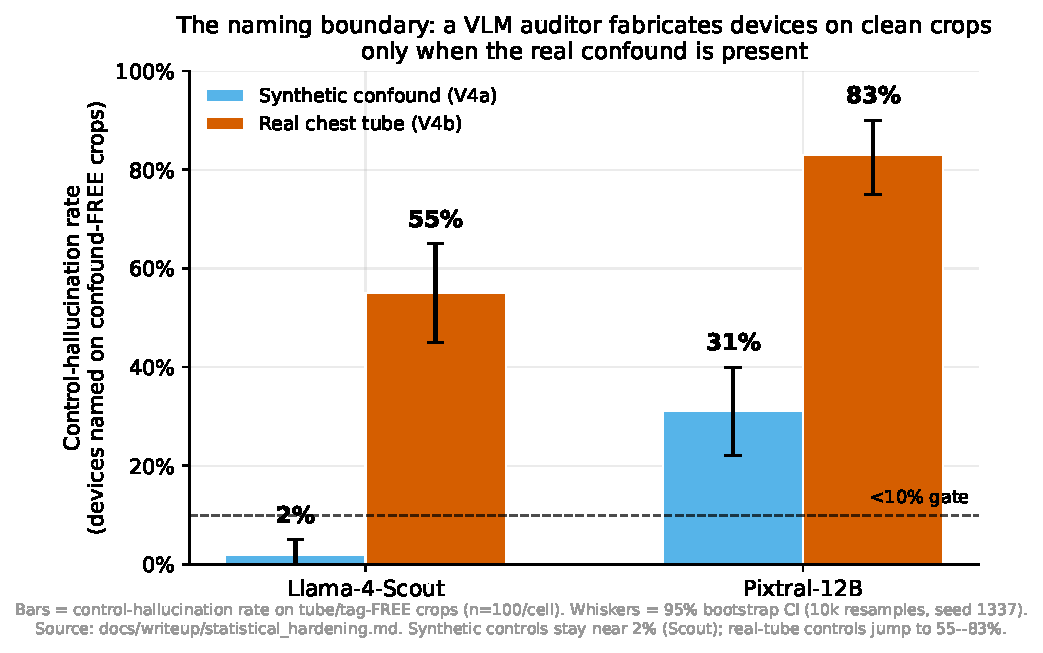
\includegraphics[width=0.9\textwidth]{figures/figure1_naming_boundary.pdf}
\caption{The naming boundary: control-hallucination (device named on a confound-free crop) for each VLM on the synthetic confound versus the real chest tube. The boundary is \textbf{per-model}, not a flat clean split: Llama-4-Scout rises from \textbf{0.02} (synthetic) to \textbf{0.55} (real); Pixtral-12B rises from \textbf{0.31} (synthetic) to \textbf{0.83} (real). Both fabricate a device on a majority of clean control crops in the real-device setting; Pixtral already fabricates on nearly a third of clean synthetic-setting crops. The $<$10\% gate is cleared only by Scout on the synthetic confound.}
\label{fig:naming_boundary}
\end{figure*}

\subsection{The Failure Is a Property of General VLMs, Not of One Model}
The obvious objection to the negative for one model is that another VLM wouldn't fail. We re-ran the \textbf{same} 200 V4b patches, the \textbf{same} blind prompt, and the \textbf{same} \texttt{names\_tube} matcher using two different VLM families
(Table~\ref{tab:multivlm}).

\begin{table}[!t]
\caption{Multi-VLM replication on the identical V4b crops, prompt, and matcher. Both models fabricate a device on a majority of clean control crops.}
\label{tab:multivlm}
\centering
\begin{tabular}{lccc}
\toprule
\textbf{model} & \textbf{precision} & \textbf{recall} & \textbf{control-hall.} \\
\midrule
Llama-4-Scout & 0.545 & 0.660 & \textbf{0.550} \\
Pixtral-12B & 0.494 & 0.810 & \textbf{0.830} \\
\bottomrule
\end{tabular}
\end{table}

They both create an invention in respect to a \emph{majority} of clean controls. The Scout re-run (0.550) recovers the original value of V4b (0.500) despite the API/decoding drift; Pixtral is much worse. Audit of the text: Scout invents particular objects (``endotracheal tube,'' ``central venous catheter'') on clean anatomy; Pixtral generates near-identical boilerplate (``linear radiopaque object\ldots appears to be a medical device or foreign body'') on \textbf{83 of 100} control images. The detection algorithm is cautious in accepting positive detections ,it does not trigger on hedged ``linear artifact'' wording --- which works to suppress false positives.

A fraud auditor using off-the-shelf general-purpose VLMs would thus issue a false alarm of the shortcutting deception on \textbf{55--83\%} of the clean images (Scout 55\%, Pixtral 83\%). This is exactly the false alarm rate that the precision vs recall gate was intended to prevent, now proven as a property common to all models. In a post-hoc bootstrap analysis with 10,000 samples and seed 1337, the difference between synthetic vs real is found to be statistically significant for both models: the 95\% confidence interval on the V4a minus V4b difference does not include zero (Scout $-0.53$ [$-0.63, -0.43$], Pixtral $-0.52$ [$-0.64, -0.40$]); Fisher's exact test rejects independence (Scout $p = 1.22\mathrm{e}{-18}$, Pixtral $p = 7.56\mathrm{e}{-14}$). It is independently validated by HalluCXR (arXiv:2605.20469) \cite{hallucxr}, which finds 61.9-82.3\% hallucination overall among six vision-language models evaluated using 856 chest X-rays, where the level of hallucination \emph{is highest on normal images} --- the same qualitative signature, in a different model population on a different task.

\subsection{What Endures the Namer's Ineffectiveness?}
Mitigation, which doesn't rely on naming, survives the real confound. DFR improves worst-group (pneumothorax-without-tube) accuracy \textbf{0.67 $\rightarrow$ 0.79 (mean across 3 seeds; a single run yields 0.83)}, while in-distribution (pneumothorax-with-tube) accuracy remains the same \textbf{0.96 $\rightarrow$ 0.96}, reducing the reliance gap \textbf{0.29 $\rightarrow$ 0.17}, without any test-distribution labels used. With 3 seeds, both independent approaches give a boost and exceed the ERM floor by 12 points, well outside of the seed variation (Table~\ref{tab:mitigation}; paired t-test on the 3 seeds: DFR-vs-ERM $p=0.030$, JTT-vs-ERM $p=0.041$ --- only for completion, since a sample size of 3 gives very little power to this test aside from detecting a large seed-consistent effect; both methods exceeding ERM in all 3 seeds by a large margin compared to the seed variation is the stronger evidence here rather than either p-value). A single auditor instruction accomplishes that end-to-end: after DFR last-layer retraining, The Grad-CAM attention moves beyond the region associated with the confound while retaining in-distribution accuracy (Figure~\ref{fig:before_after}).

\begin{table}[!t]
\caption{Mitigation across 3 seeds (mean $\pm$ std). Worst-group and in-distribution (ID) accuracy and the reliance gap, for the real tube and the synthetic tag.}
\label{tab:mitigation}
\centering
\begin{tabular}{llccc}
\toprule
\textbf{confound} & \textbf{method} & \textbf{worst-group} & \textbf{ID} & \textbf{reliance gap} \\
\midrule
tube & ERM & $0.672 \pm 0.022$ & $0.959 \pm 0.002$ & $0.287 \pm 0.025$ \\
tube & JTT & $0.791 \pm 0.047$ & $0.940 \pm 0.019$ & $0.149 \pm 0.031$ \\
tube & DFR & $0.790 \pm 0.036$ & $0.964 \pm 0.007$ & $0.174 \pm 0.029$ \\
tag & ERM & $0.500 \pm 0.000$ & $0.940 \pm 0.000$ & $0.440 \pm 0.000$ \\
tag & JTT & $0.608 \pm 0.018$ & $0.531 \pm 0.016$ & $-0.077 \pm 0.025$ \\
tag & DFR & $0.609 \pm 0.022$ & $0.603 \pm 0.014$ & $-0.006 \pm 0.024$ \\
\bottomrule
\end{tabular}
\end{table}

\begin{figure*}[!t]
\centering
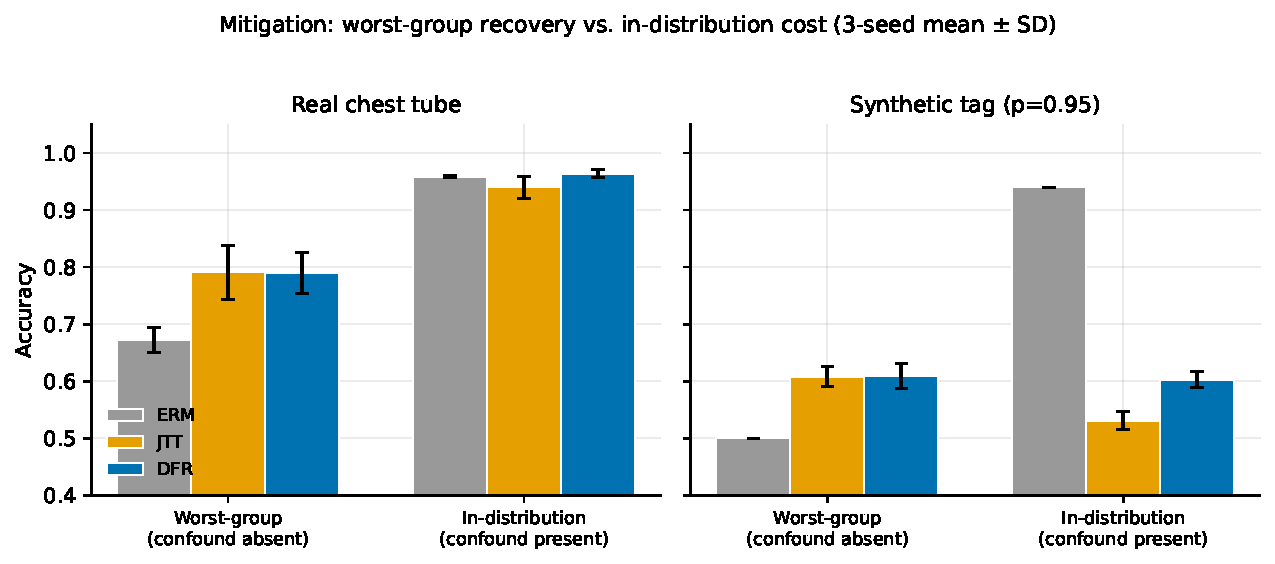
\includegraphics[width=0.85\textwidth]{figures/fig6_mitigation_comparison.pdf}
\caption{Mitigation comparison (Table~\ref{tab:mitigation}): worst-group and in-distribution accuracy for ERM, JTT, and DFR on the real tube confound and the synthetic tag confound, 3-seed mean $\pm$ std. On the tube, DFR and JTT both clear the ERM worst-group floor by roughly 12 points while preserving in-distribution accuracy; on the tag, the same procedures collapse in-distribution accuracy alongside the reliance gap, the cautionary result discussed in \S\ref{sec:supporting}.}
\label{fig:mitigationbar}
\end{figure*}

\begin{figure*}[!t]
\centering
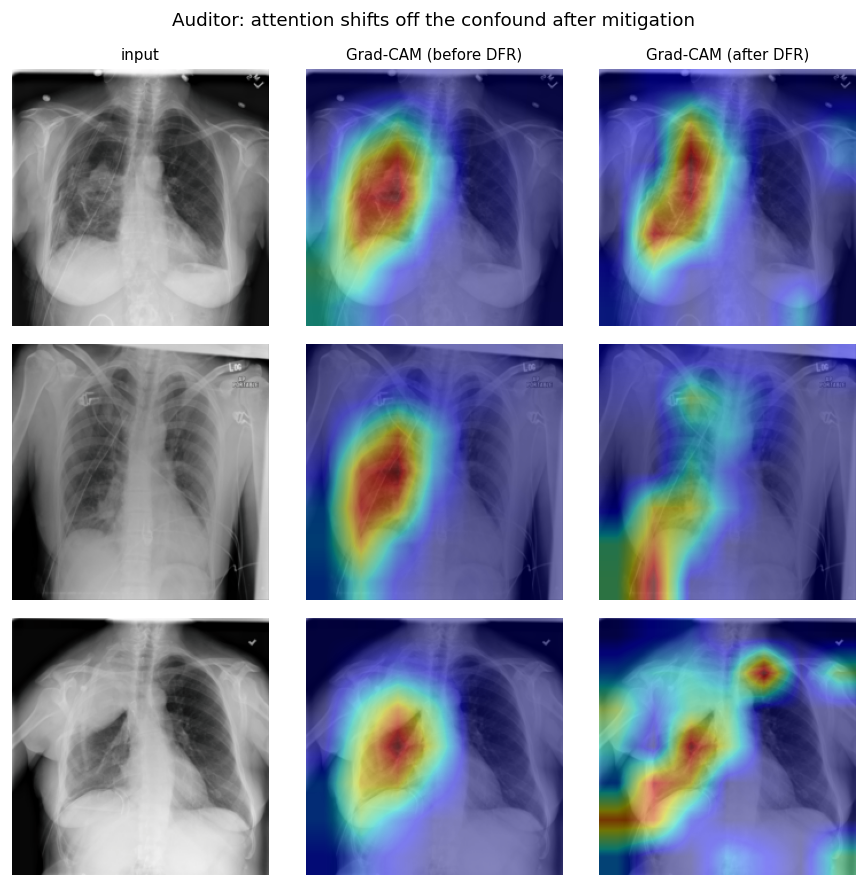
\includegraphics[width=0.9\textwidth]{figures/auditor_before_after_tube.png}
\caption{Before/after Grad-CAM on the actual tube model, which has been generated via a single auditor action (detect$\rightarrow$mitigate). Post DFR last layer retraining, attention expands out of the confound-relevant region while maintaining in-distribution accuracy (0.96$\rightarrow$0.97 for this single demo) and improving worst-group accuracy.}
\label{fig:before_after}
\end{figure*}

This is the story of the synthetic label which tells the side of caution; while the gap closes (0.44 $\rightarrow$ 0.02), the in-distribution accuracy drops from 0.94 to 0.62. To disprove the temptation of ``backbone is hollow'' by conducting a linear probe test deliberately to do that, the result of AUC for probe is \textbf{0.690}, which is greater than random guess (0.50), but below clean baseline (0.845). Shortcut usage \textbf{hampers but does not prevent} acquisition of essential features, and the hampering is strength-dependent.

Cross-site, there is a genuine discrepancy which is not accounted for by the shortcut. NIH reference AUC \textbf{0.842} drops to PadChest \textbf{0.650}, which amounts to a decrease of \textbf{0.192} (95\% CI \textbf{[0.159, 0.225]}, stratified bootstrap, 2,000 repetitions over the images from the test set), exactly what Zech et al.\ \cite{zech2018} found --- a genuine effect, not an edge case. Target adaptation based on supervised learning recovers \textbf{$+0.082$} --- but this is just last layer fine-tuning on \emph{labeled} PadChest, so it would be helpful even without any shortcut. The truth, zero-shot source domain adaptation using no target labels, yields \textbf{$+0.005$} (95\% CI \textbf{[$-0.018$, $+0.028$]}, same bootstrap procedure). Since the confidence interval contains a large negative value for recovery, as well as zero, the estimate is not sufficient to demonstrate any effect --- yet it is also sufficiently large such that it does not rule out a small-to-moderate effect ($\sim +0.03$ AUC): this is an \textbf{underpowered null hypothesis}, not a \emph{tight} null hypothesis, and we report on it as such, not as proof that a known and real source-side shortcut can't help transfer learning. The reduction of 0.192 is distribution shift and is not attributable to any cause within the current experimental design, although shortcuts are one of many potential candidates.

\begin{figure*}[!t]
\centering
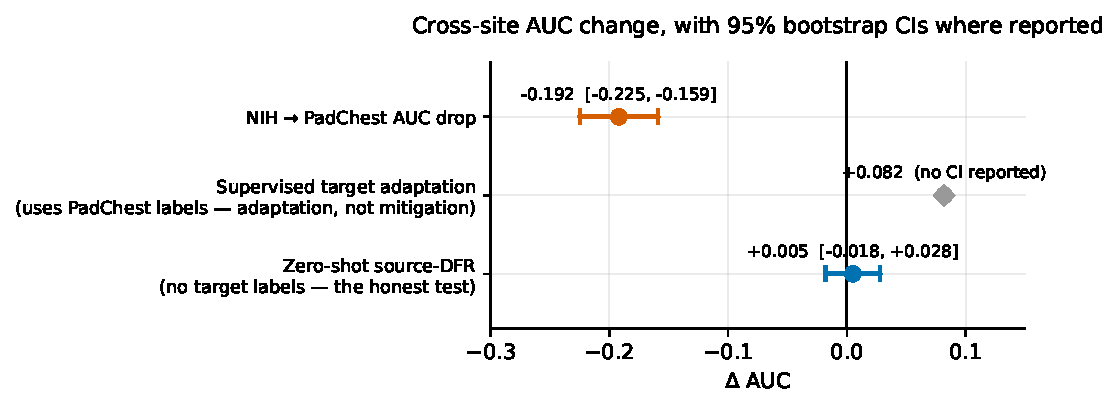
\includegraphics[width=0.85\textwidth]{figures/fig5_crosssite_forest.pdf}
\caption{Cross-site AUC change from NIH to PadChest, with 95\% bootstrap CIs where reported. The baseline drop ($-0.192$) is real and Zech-magnitude. Supervised target adaptation ($+0.082$, no CI reported) uses PadChest labels and licenses no mitigation claim. The zero-shot, label-free source-DFR test ($+0.005$, 95\% CI [$-0.018$, $+0.028$]) is the honest test of whether the known source-side shortcut explains the gap: its interval includes zero and excludes a large recovery.}
\label{fig:forest}
\end{figure*}

\subsection{Mechanism --- Why Naming Breaks}
\label{sec:mechanism}
V4a and V4b are two points, not a mechanism. Two follow-up experiments ask \emph{why} naming breaks: whether fabrication is driven by the confound's \textbf{visibility}, and whether it is grounded in the image at all.

\subsubsection{Experiment 1 --- the difficulty curve is a recall cliff, not a hallucination cliff}
The intuitive hypothesis is that fabrication rises as the confound gets fainter. We tested it directly by sweeping the synthetic tag's opacity across $\{0.25, 0.5, 0.75, 1.0\}$ and re-scoring both models with the unchanged pipeline ($n = 200$ crops per cell, 100 positive + 100 control), shown in Table~\ref{tab:difficulty}.

\begin{table}[!t]
\caption{Difficulty curve: sweeping synthetic-tag opacity. Reducing visibility produces a recall cliff while control-hallucination stays flat.}
\label{tab:difficulty}
\centering
\begin{tabular}{llccc}
\toprule
\textbf{opacity} & \textbf{model} & \textbf{precision} & \textbf{recall} & \textbf{control-hall.} \\
\midrule
0.25 & scout   & 0.600 & 0.030 & 0.020 \\
0.25 & pixtral & 0.420 & 0.210 & 0.290 \\
0.50 & scout   & 0.963 & 0.520 & 0.020 \\
0.50 & pixtral & 0.588 & 0.400 & 0.280 \\
0.75 & scout   & 0.978 & 0.900 & 0.020 \\
0.75 & pixtral & 0.556 & 0.400 & 0.320 \\
1.00 & scout   & 0.978 & 0.900 & 0.020 \\
1.00 & pixtral & 0.626 & 0.520 & 0.310 \\
\bottomrule
\end{tabular}
\end{table}

Reducing visibility produces a \textbf{recall cliff} --- Scout's recall collapses 0.90 $\rightarrow$ 0.52 $\rightarrow$ 0.03 between opacity 0.75, 0.5 and 0.25 --- while \textbf{control-hallucination stays flat}: $\sim$0.02 for Scout and $\sim$0.28--0.32 for Pixtral across \emph{every} opacity level. Faintness makes the model miss the confound; it does not make the model invent one.

This \textbf{rules out visibility as the bridge} from V4a's 0.02 hallucination to V4b's 0.50--0.83. Whatever separates the synthetic tag from the real tube, it is not how hard the confound is to see. The revised working hypothesis is that fabrication tracks the \textbf{anatomical plausibility of the confound category}: a synthetic tag is never mistakable for anatomy at any opacity --- it is either seen or not, with no ambiguous middle --- whereas a real device sits inside a space of plausible near-misses (other lines, catheters, vessels, fissures, rib edges) that a VLM's medical-image priors can generate confident boilerplate about.

\begin{figure*}[!t]
\centering
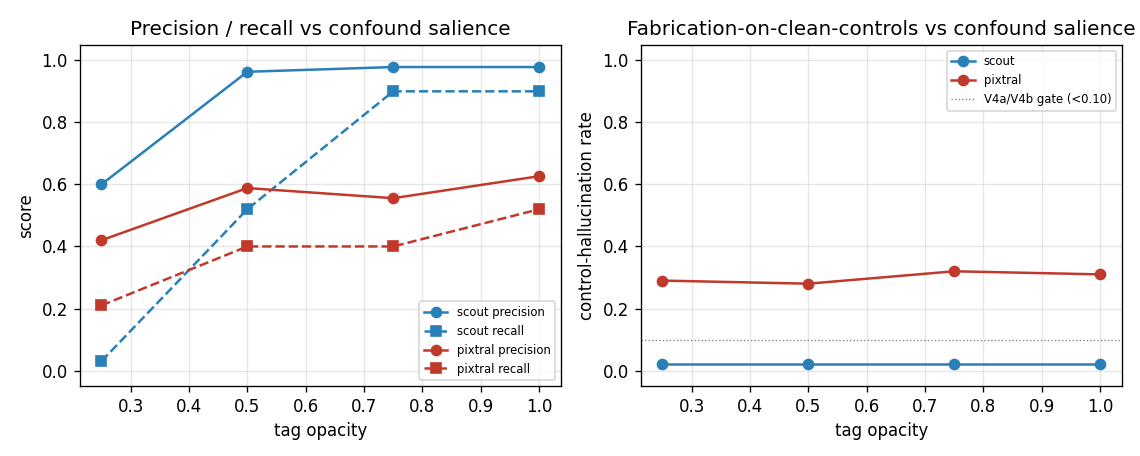
\includegraphics[width=0.85\textwidth]{figures/exp1_difficulty_curve.png}
\caption{Naming-difficulty (opacity) sweep for the synthetic tag (Table~\ref{tab:difficulty}). Reducing opacity produces a recall cliff for Scout ($0.90 \rightarrow 0.52 \rightarrow 0.03$) while control-hallucination stays flat ($\sim$0.02 Scout, $\sim$0.28--0.32 Pixtral) at every opacity level: faintness makes the model miss the confound, it does not make it invent one.}
\label{fig:difficulty}
\end{figure*}

\begin{figure*}[!t]
\centering
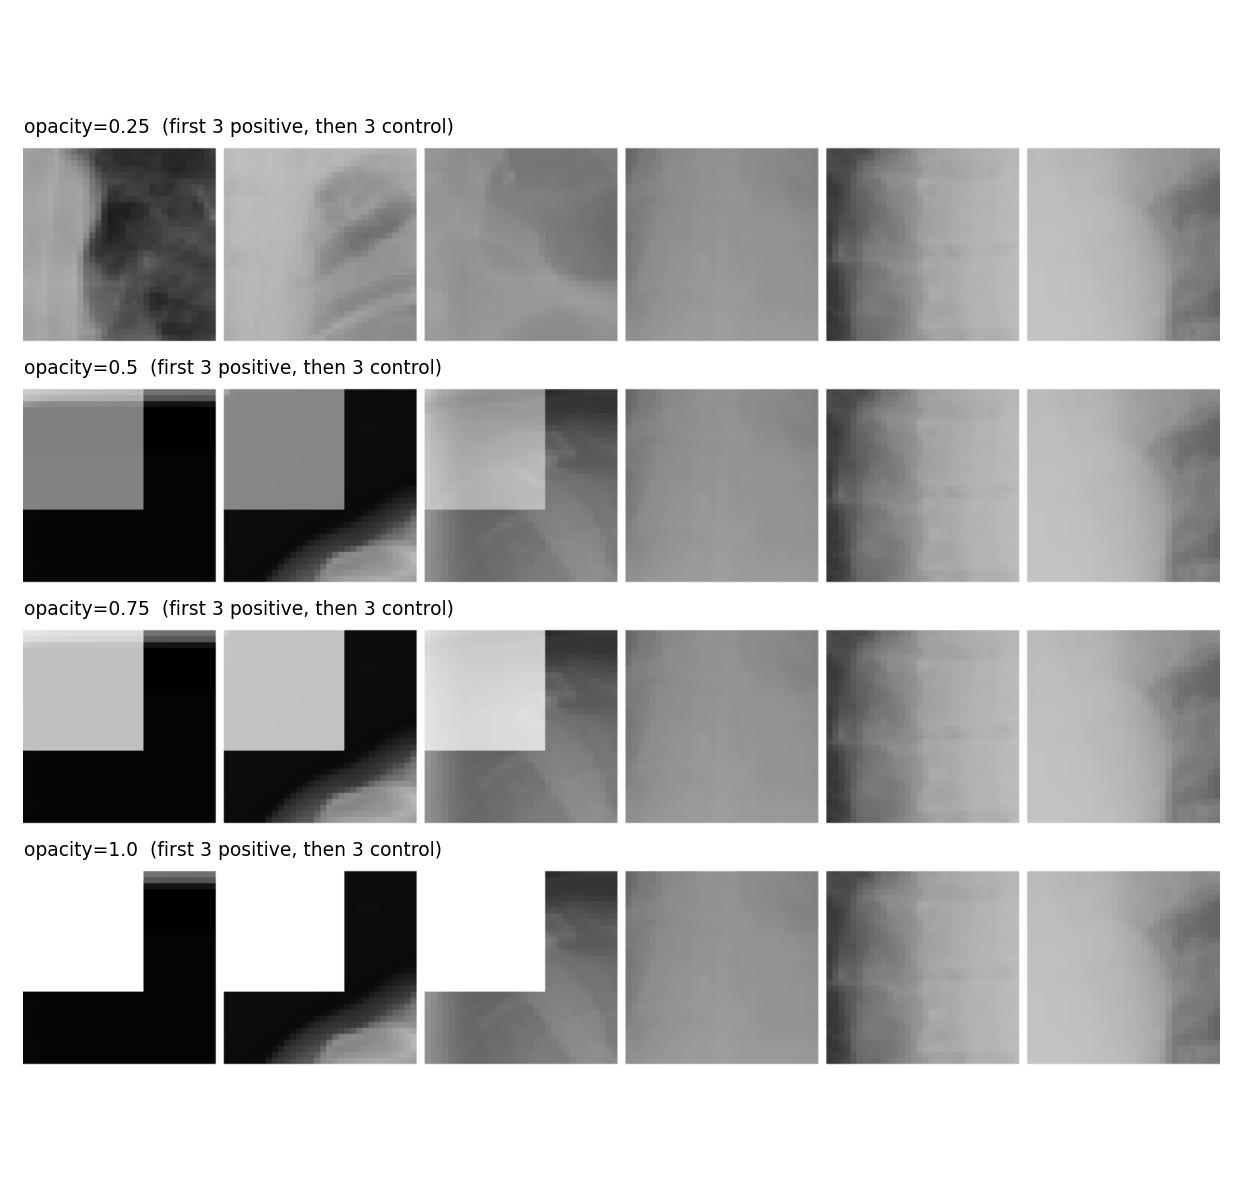
\includegraphics[width=0.85\textwidth]{figures/exp1_contact_sheet.png}
\caption{Representative synthetic-tag crops across the opacity levels swept in Table~\ref{tab:difficulty} (0.25--1.0), illustrating the visual difficulty gradient underlying the recall cliff in Figure~\ref{fig:difficulty}.}
\label{fig:contactsheet}
\end{figure*}

\subsubsection{Experiment 2 --- fabrication is based on grounded interpretation, not recitation from memory}
This alternative hypothesis posits that the VLM is not even looking at the image itself, which is not implausible in light of Lotfinia et al.\ (arXiv:2606.17710) \cite{lotfinia2026}, who demonstrate that VLMs can respond to chest-radiograph question answering from language priors without even paying attention to the image. Should V4b's descriptions be completely dependent on language priors rather than visual input, the auditor's naming would be meaningless, regardless of its accuracy.

To test this we ran three types of per-crop perturbation, relative to each VLM's unperturbed-crop baseline description: occlusion of the \textbf{relevant} region of the image, occlusion of an \textbf{irrelevant} region, equally-sized, or \textbf{substitution} with another same-kind crop. Change judgments are parsed into direction categories because the total proportion of change judgments conflates two opposite results: \textbf{pos$\rightarrow$neg} (device named correctly before, but not after the edit) supports grounding; \textbf{neg$\rightarrow$pos} (a \emph{new} device is detected \emph{after} the edit) represents fabrication displaced. All 12 cells are complete at $n = 100$ (Table~\ref{tab:grounding}).

\begin{table}[!t]
\caption{Grounding experiment: verdict changes by direction, per dataset/condition/model, at $n = 100$.}
\label{tab:grounding}
\centering
\footnotesize
\begin{tabular}{lllcccc}
\toprule
\textbf{dataset} & \textbf{condition} & \textbf{model} & \textbf{pos$\rightarrow$neg} & \textbf{neg$\rightarrow$pos} & \textbf{unch.} & \textbf{chg rate} \\
\midrule
v4a & relevant   & scout   & 19 & 5  & 76 & 0.24 \\
v4a & relevant   & pixtral & 25 & 22 & 53 & 0.47 \\
v4a & irrelevant & scout   & 16 & 5  & 79 & 0.21 \\
v4a & irrelevant & pixtral & 27 & 24 & 49 & 0.51 \\
v4a & swap       & scout   & 8  & 8  & 84 & 0.16 \\
v4a & swap       & pixtral & 27 & 23 & 50 & 0.50 \\
v4b & relevant   & scout   & 61 & 1  & 38 & 0.62 \\
v4b & relevant   & pixtral & 66 & 5  & 29 & 0.71 \\
v4b & irrelevant & scout   & 30 & 4  & 66 & 0.34 \\
v4b & irrelevant & pixtral & 13 & 2  & 85 & 0.15 \\
v4b & swap       & scout   & 20 & 21 & 59 & 0.41 \\
v4b & swap       & pixtral & 17 & 17 & 66 & 0.34 \\
\bottomrule
\end{tabular}
\end{table}

The artifact in the measurement of the occluded tag is that almost all of this table needs to be interpreted carefully. The flat gray fill used to occlude the tag is routinely classified by the VLM as ``a gray rectangular object\ldots{} artificial and not part of the patient's anatomy\ldots{} a label or marker''---language which triggers the exact \texttt{names\_confound} condition designed into the occlusion. Checking a few at random confirms it: \textbf{76 of 100} Scout descriptions under V4a \emph{relevant} occlusion still show up as positive, as many as the \texttt{unchanged} count, and examining them reveals that the model is interpreting the \textbf{patch used for the occlusion}, not the remaining tag content. Thus, \textbf{the V4a \texttt{relevant} numbers underestimate actual grounding}, and the comparison between V4a and V4b does not provide an answer here---the measurement is biased toward \texttt{unchanged} for V4a in a way that it is not for V4b.

\textbf{The evidence supporting the conclusion is the V4b-internal contrast.} The matcher used by V4b (\texttt{names\_tube}) needs specific device-related vocabulary --- something that is not similar to a plain gray rectangle in the way an ``artificial marker'' is --- and thus, its vulnerability to the artifact is much smaller (only 38 out of 100 Scout descriptions are still positive after V4b-specific occlusion, compared to V4a's 76). In the case of V4b, both conditions involve the same matcher operating on the same data set, with the only difference being the \emph{location} of the occluder:
\begin{itemize}
\item Occluding the \textbf{region containing the tube} reduces the device name recognition rate: pos$\rightarrow$neg \textbf{61/100} (Scout), \textbf{66/100} (Pixtral).
\item Occluding an equal-area \textbf{irrelevant} region reduces it far less: pos$\rightarrow$neg \textbf{30/100} (Scout), \textbf{13/100} (Pixtral).
\end{itemize}

Device-name identification follows the tube pixel locations. ``V4b fabrication is pure image-independent prior-emission'' is unfounded. The reconciled device name generation mechanism, analyzed with regard to the 50--83\% control-hallucination on clean crops: VLM generates strong \textbf{device-presence prior} \emph{and} grounds this prior in the salient region --- reading of a real device when a device is present, and \textbf{false-positive hallucinating a device in ambiguous normal anatomy} when there is no device at all. It is the prior-emitter-based overreading of an ambiguous salient region, which is neither a mindless recitation nor clean perception, and aligns with the discovery in Experiment 1 that plausibility, and not visibility, drives the device naming process. (Supporting but not a load-bearing evidence: the symmetry of V4b swap condition --- 20/21 Scout, 17/17 Pixtral --- and \texttt{text-identical-rate} = 0.0 for each cell combination shows that verbatim recitation does not cause the failure. A texture-matched occluder should be used in replication for the V4a arm.)

\begin{figure*}[!t]
\centering
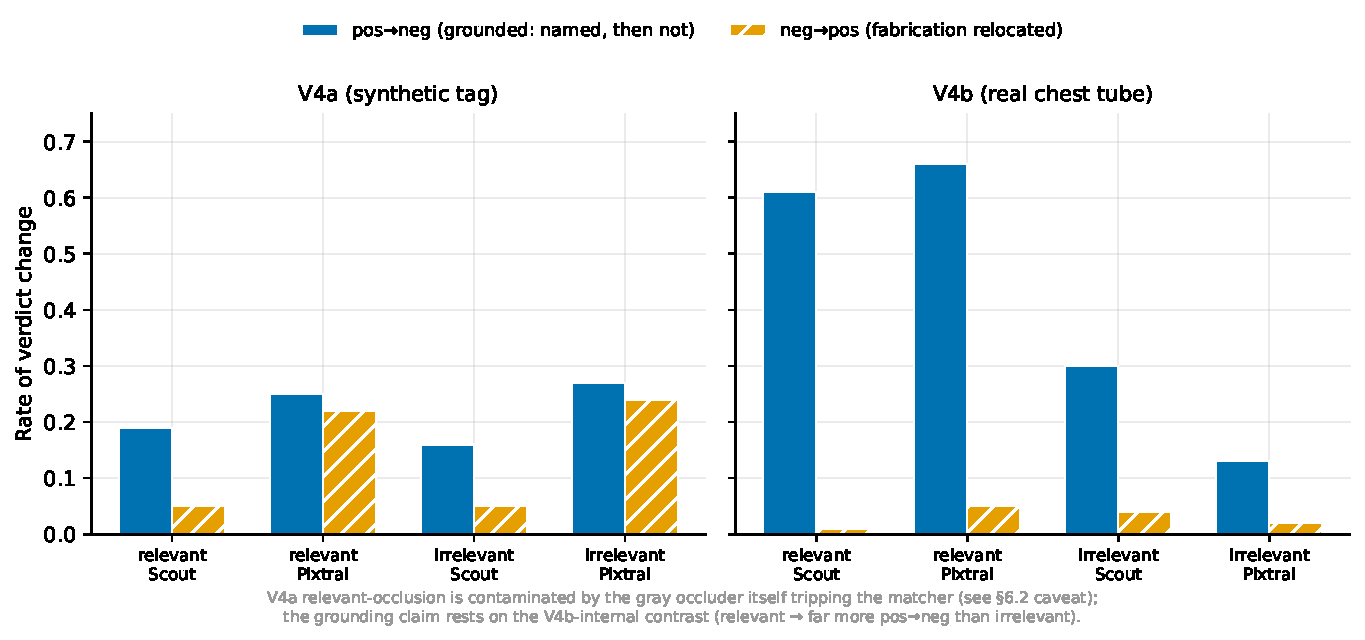
\includegraphics[width=0.85\textwidth]{figures/fig4_occlusion_grounding.pdf}
\caption{Image-independence (occlusion/swap) study (Table~\ref{tab:grounding}). pos$\rightarrow$neg (named at baseline, not after) is consistent with grounding; neg$\rightarrow$pos is fabrication merely relocated. Within V4b, occluding the tube region drops device-naming far more (61/100 Scout, 66/100 Pixtral) than occluding an equal-area irrelevant region (30/100 Scout, 13/100 Pixtral); the V4a \texttt{relevant} condition is contaminated by the gray occluder itself tripping the \texttt{names\_confound} matcher and should be read with that caveat.}
\label{fig:occlusion}
\end{figure*}

\subsection{Specialist VLM}
\label{sec:specialist}
This V4b gate mechanism, however, was developed for general-purpose VLMs alone, which opens another possibility for avoiding the failure: a radiology-tuned VLM with the device vocabulary absent in general models might get through the gate where the latter failed. This did not happen, but the way this failure happens is what matters. An additional six models have been tested on the \textbf{same} V4a/V4b images and the same blind prompt (confirmed with byte check to be the same as the general group's), with scoring being done with the project's matchers. Three of them are to be reported; \textbf{the other three cannot be considered model outputs because they contain bugs of the harness output}, and their score zeros are not to be interpreted as such; \textbf{phi3.5-vision} has returned an empty string in response to all 200 crops of both arms; \textbf{qwen2.5-vl-3b} refused to generate a response on 164/200 V4a crops --- the image never reached the model; \textbf{MedGemma} generated 400 empty responses due to a quantized-vision-tower bug, diagnosed separately, with a re-run pending. Reporting any of these as a naming failure would be a fabrication of the opposite kind. \emph{Three models reported; three excluded for harness output bugs.}

The three problematic models --- qwen2.5-vl-7b, CheXagent-2-3B, and chexagent-8b --- are cleanly divided along one dimension: those which \textbf{over-name}, or \textbf{under-name}, the device. Both types fail both V4b gates, but for different reasons, and this divide is the contribution.

\textbf{Over-naming is the default tendency of general VLMs, and it is not a small-model artifact.} The V4b fabrication that prompted the shift to a new criterion was general-VLM behavior: in tubes-free controls, Llama-4-Scout hallucinates a device in \textbf{0.55} clean crops (95\% bootstrap CI [0.45, 0.65]), while Pixtral-12B hallucinates in \textbf{0.83} ([0.75, 0.90]). qwen2.5-vl-7b --- a \emph{larger} general VLM, and the sole new model with a substantial signal (V4a precision \textbf{0.63}, recall \textbf{0.33}) --- over-names just as readily: the control-hallucination in its V4b gate is \textbf{0.74}. Over-naming is not an artifact of the 12B-and-under general models that first showed it; it persists at 7B in a fresh model family, at a rate that still fails the $<$0.10 control-hallucination bar sevenfold.

\textbf{The medical specialist under-names --- a structural zero.} CheXagent-2-3B does not respond in free text; it generates its own referring expression grounding tokens (\texttt{<|ref|> foreign object <|/ref|> <|box|>\ldots<|/box|>}). Evaluated with a grounding-aware matching criterion that holds it to the \emph{same} genericness standard as the general-purpose models, it performs well above the precision bar set for V4a (precision \textbf{0.9663}, recall \textbf{0.86}, control-hallucination \textbf{0.03}) --- close to the precision bar and far beneath the fabrication bar. With V4b it scores exactly \textbf{0.0 / 0.0 / 0.0}. This is not a perception failure: CheXagent generated a grounded label for \textbf{100/100} V4b tube-positive crops. It is a \emph{taxonomical} failure. The entire grounded vocabulary that it has ever exhibited is $\{$foreign object, diaphragm, other lesion, artificial object, aortic enlargement, mediastinal$\}$ --- there is \textbf{not one device-specific class} among all of its possible output classes: there is no term for tube, catheter, line, drain, or wire, in either dataset. The specialist localizes the tube but \emph{cannot name it}, because ``name it as a device'' is simply not a possibility afforded to it taxonomically. Where the general VLMs fail V4b by saying too much on clean crops, the specialist fails by having no word for the thing it is grounding on.

\textbf{Under-naming holds up under a 3B$\rightarrow$8B scale-up.} chexagent-8b, the larger brother, responds using radiology-report free text, instead of grounded tokens, and achieves a score of \textbf{0.0 / 0.0 / 0.0} on both parts; its free text never matches the vocabulary that the matcher relies on, and there are no corresponding control hits. Thus, under-naming is not due to some 3B size limitation --- it holds through a 3B$\rightarrow$8B scale-up --- but is simply an intrinsic feature of the vocabulary design for the expert's output space. Naming a device is a vocabulary-design decision made upstream of scale.

\textbf{One warning about taking an over-clean interpretation.} ``Specialist under-names, general over-names'' is the key axis, but it is not the \emph{only} key axis, and the general models are not uniformly safe where the specialist fails to name. In the ``clean'' \textbf{synthetic} V4a controls, hallucination is model-dependent: Scout hallucinates on \textbf{0.02} of clean crops ([0.00, 0.05]), but Pixtral on \textbf{0.31} ([0.22, 0.40]), which represents the per-model fabrication \emph{floor}, irrespective of whether the model is a domain specialist or general. ``Synthetic naming is safe if it is done using the general model'' is the Scout story; another general VLM hallucinates on a third of the same ``easy'' controls. In other words, the auditor's reliability depends on the specific model used for both axis --- the amount of over-naming on clean crops \emph{as well as} the model vocabulary's ability to name the target --- and neither is predetermined by the specialist-general label.

\begin{figure*}[!t]
\centering
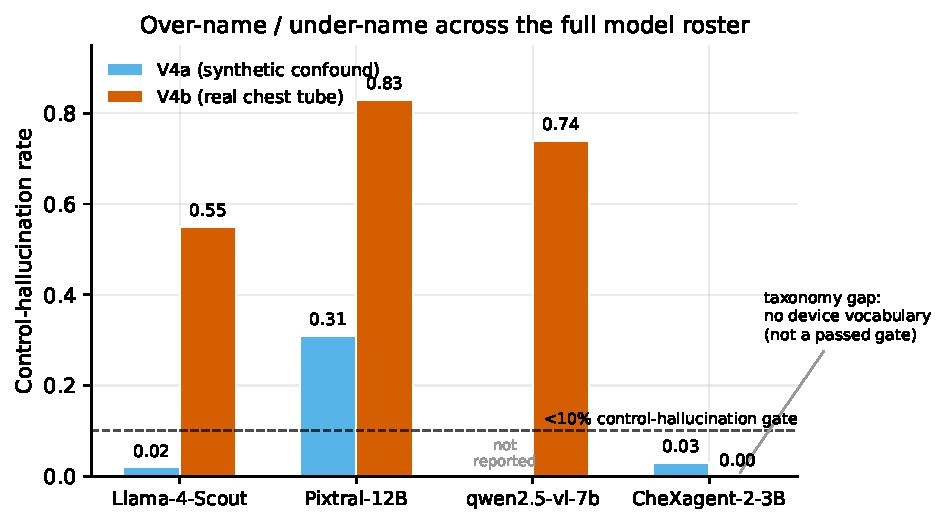
\includegraphics[width=0.85\textwidth]{figures/fig3_overname_underrname_roster.pdf}
\caption{Control-hallucination on confound-free crops across the full tested model roster, synthetic (V4a) vs.\ real chest tube (V4b), extending Figure~\ref{fig:naming_boundary} to the full roster. Llama-4-Scout and Pixtral-12B both fabricate on a majority of clean real-device crops; qwen2.5-vl-7b over-names just as hard (0.74) despite being a larger, newer general model. CheXagent-2-3B's 0.0 on V4b is a taxonomy gap --- its output vocabulary has no device class --- not a passed gate.}
\label{fig:roster}
\end{figure*}

\subsection{Supporting Evidence and Robustness}
\label{sec:supporting}
There are five VLM-independent studies that test the robustness of the results presented above. None is a headline; each one either bolsters a finding via an independent line of reasoning or constrains an alternative explanation.

\textbf{The tube shortcut is insensitive to severity (underpowered).} When the 94 shared pneumothorax-positive test images are stratified by the median bounding-box area, and balanced between tiers, there is perfect accuracy for the presence of a tube, at \emph{any} lesion size, while accuracy is poor without a tube, at \emph{any} lesion size (gap for low-severity 0.400 at $n$=20; gap for high-severity 0.4375 at $n$=16). The gap is large in both strata, thus ruling out any simple disease-burden proxy, but at $n$=16--20 per group it is underpowered to tell the difference between invariance and a genuine severity effect, so the invariance claim is disallowed; what remains is that even low-severity examples show a large gap --- the shortcut is \textbf{device-keyed, not disease-burden-keyed}.

\textbf{The DFR result is a floor, not a ceiling.} One version of DFR (with regularization parameter $C$ chosen by 5-fold cross-validation and average weights taken from 10 balanced draws) is a strict improvement over single-draw DFR on the tube problem (worst-group 0.84$\rightarrow$0.93, ID 0.965$\rightarrow$0.998, gap 0.12$\rightarrow$0.07), thereby showing that the DFR result in question is not a result of good hyperparameter tuning. On the synthetic tag problem it restores some ID accuracy (0.594$\rightarrow$0.687), but stays far away from the 0.94 baseline value; the tag ``closing'' the gap is partially an effect of the symmetrical tagged/untagged validation construction, documented as an anomaly, and the tube result is the one we defend.

\textbf{Redundant encoding of site identity (another version of the V6 null)}. A hospital classifier distinguishes NIH from PadChest by projecting from the frozen penultimate features using AUC \textbf{0.9993}, but when the hospital direction is projected out and the frozen disease head is scored, there is no change to disease AUC \textbf{(0.6436 $\rightarrow$ 0.6436, $\Delta$ 0.000)}. Even using the projected features with a new probe achieves AUC 0.9990 --- a single rank-1 projection does not reduce the site information very much, correcting an over-claim made previously. The disease AUC null holds regardless, because it is measured on the frozen head.

\textbf{Label-free OOD attribution: the synthetic-vs-real asymmetry.} Extending the zero-shot source-DFR experiment to the synthetic label, not only does tag-based mitigation fail to transfer, it actually \emph{hurts} the transfer ($-0.083$ for PadChest, vs $+0.005$ null for the tube). The \emph{pure} synthetic shortcut at $p$=0.95 is almost a total representation override; while the tube model learns the disease along with the shortcut, the tag model almost entirely ceases to learn the disease. Synthetic shortcuts confirm the \emph{methodology}, but systematically \emph{exaggerate} the problem relative to real-world examples, and should not be extrapolated to real shortcuts without the real-arm check.

\textbf{Reliance depends on: the correlation sweep.} Scanning the strength of the correlation $p$ at \textbf{a single training seed per point} (a limitation maintained in the Limitations section), the reliance gap increases monotonically \textbf{across the following five single-seed runs} --- 0.000 ($p$=.6) $\rightarrow$ 0.010 $\rightarrow$ 0.075 $\rightarrow$ 0.294 $\rightarrow$ 0.440 ($p$=.95) --- a pattern, albeit without yet a replicated result at the training level, that has an \textbf{onset threshold}, with a correlation too weak below $p \approx 0.7$ for the model to take advantage of and learn real signal (test AUC $\approx$ 0.83). The cost of DFR in-distribution follows this strength dependence, with negligible costs where the shortcut does not exist and substantial costs where the shortcut was allowed to take over. DFR recovery was performed on 3 seeds across each of the frozen per-$p$ checkpoints; all single-seed values lie within roughly one standard deviation of these means, so the sweep's conclusions do not hinge on the seed (the \emph{training}-seed variance of the gaps themselves is not claimed).

\begin{figure*}[!t]
\centering
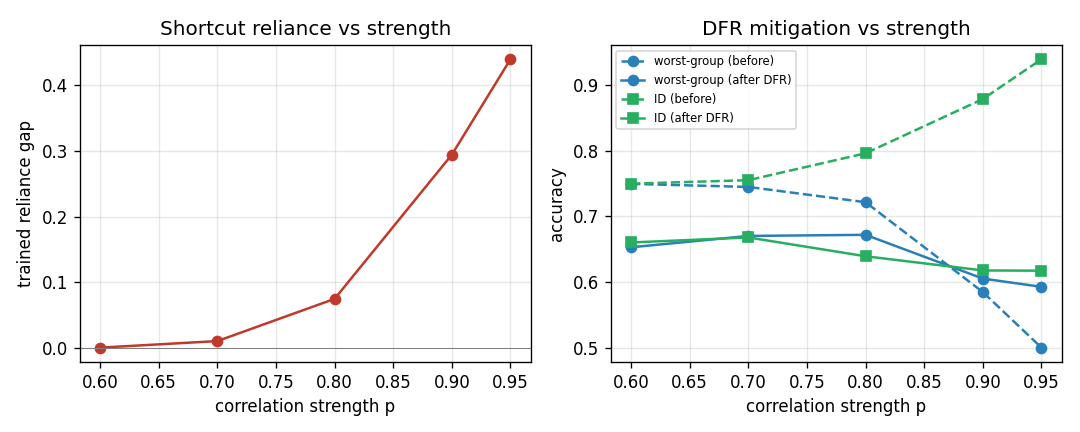
\includegraphics[width=0.85\textwidth]{figures/sweep_figure.png}
\caption{Relevance gap in relation to injected tag correlation $p$ (1 train seed per point). Relevance is close to zero until $p \approx 0.7$, after which it increases sharply to reach the 44pp figure at $p=0.95$.}
\label{fig:sweep}
\end{figure*}

\textbf{Fifth analysis, shown as blocked.} The severity-\textbf{aware} mitigations were not performed: there are severity annotations only for the 94-image test split, and no proxy was fabricated. It is reported as blocked rather than omitted.

% =====================================================================
\section{Discussion}
The key point of the paper is a boundary condition: the blind, universal VLM naming applies to unambiguous shortcuts and breaks down --- through faking --- for ambiguous shortcuts of a certain type. Both mechanisms experiments clarify \emph{on which} axis the boundary condition applies. Visibility is not it: darkness leads to a recall cliff, not hallucination cliff (Experiment 1). The boundary condition is plausibility. Synthetic corner tags cannot be confused with anatomy no matter what transparency level and thus, the model either recognizes them or does not; in contrast, chest tubes share the space with various lines, catheters, blood vessels, lung fissures, and rib edges that the device-centric VLM is prepared to name using its templates. Furthermore, the Experiment 2 rules out the possibility of the deflationary interpretation where the VLM does not pay any attention to the existence of the image at all: device naming is correlated with tube pixels (blocking of the tube decreases the likelihood of device naming by almost twice as much as blocking of some unrelated part of the same size). In other words, the breakdown is neither a simple repetition nor correct interpretation --- it is \textbf{an over-interpretation of ambiguous salient parts}.

Our problem is \textbf{the over-name / under-name axis} because each of them has its unique penalty for an auditor. Under-naming (miss) is graceful --- it was proven in Experiment 1: as the confound disappears, the model does not name it anymore and recall is penalized more than precision due to that. Over-naming (fabrication), on the other hand, is a more harmful mode of failure: a tool that fabricates a chest tube from the empty radiograph will force a physician to follow a fictitious shortcut, and, according to our experiment, 55\%-83\% clean crops are prone to hallucinations on average. This is why the design featured control hallucination as a \emph{gate} instead of being a metric and why the truth is that general-purpose VLMs cannot be safely used to audit clean images without a gate. The nature of the boundary condition being per-model (Figure~\ref{fig:naming_boundary}: Scout hallucinates on 2\% of synthetic controls while Pixtral hallucinates on 31\%) reinforces the conclusion: even in ``simple'' synthetic case, one of the two general-purpose models does not pass the gate.

The fact of the survival of the naming failure plays an important role in the interpretation of the contribution. The mitigation is robust, realistic and specifically designed to not depend on the faulty naming procedure because none of the methods of the mitigation pipeline uses the VLM module, so the naming-off is automatically included into the code and not done as an additional experiment. DFR increases the accuracy for the worst group from 0.67 to 0.79 (mean over 3 seeds) in the true tube while keeping the in-distribution accuracy with no target distribution labels, and two completely independent methods give the same number beyond the seed variance. We pay special attention to the crucial statistics --- 0.79 is the mean over 3 seeds; the larger 0.83 number is given explicitly as a single-draw result. The reason is clear --- presenting the fortunate draw as the final one would constitute an overestimation of the result, which was avoided intentionally by the paper's method. And finally, the synthetic tag gives the complementing warning --- the complete shortcut at $p$=0.95 is so dominant that its absence leaves too few disease signal left, and that is the reason why the synthetic confounds validate the \emph{method} but overestimate the \emph{phenomenon}.

This is where the cross-site effect comes into play, where we will most strongly resist the siren's call. Indeed, there is a real 0.192 US-to-Spain AUC loss, Zech magnitude, and it is very tempting to report the loop as ``validated cross-site.'' It is not. The supervised recovery effect ($+0.082$) makes use of the PadChest labels and would be quite valuable if there wasn't already a shortcut available; the zero-shot source-DFR test effect --- diminish the \emph{known} tube shortcut at NIH only, leaving the target labels alone --- returns $+0.005$ (95\% CI [$-0.018$, $+0.028$]), an effect size estimate that is indistinguishable from zero, in an interval so wide that it cannot rule out even a small-to-moderate effect. Diminishing a known shortcut did not measurably diminish the cross-site discrepancy in this test, so the distribution shift is cross-site and cannot be attributed to the shortcut effect --- recognizing the sensitivity of the test to even a modest effect was weak. Representation-level control effects do not help but instead hurt here: site membership is almost completely de-codable (AUC 0.9993) and yet the frozen disease head cannot decode it ($\Delta$ 0.000 after projecting site out), and thus the two things that one would expect first --- a head riding a site signal and a covariate shift solved by label-free adaptation --- are both near zero, and the majority of the gap remains unexplained. The clinically load-bearing consequence is that ``fix the known shortcuts'' is \emph{not} sufficient due diligence before cross-site deployment.

Finally, scope honesty. This is a pathological condition (pneumothorax), one primary corpus (NIH) along with one secondary corpus (PadChest), one confounding instrument in the real world (chest tube) with annotation independent of experts, and VLMs in general (not specialized). These two mechanism experiments bounded the boundary of visibility and grounding but did not map out the boundary on the plausibility dimension suggested by the mechanism --- we know what is nameable when the marker is obvious and what isn’t when the instrument is subtle, but not how much of it lies in between. The pre-registration stopping criterion influenced the gate decision itself --- a failure at V4b following success at V4a made the decision to move away from this option immediately and explicitly, but not iterated on it --- but it does not prohibit a relatively cheap follow-up ablation (abstention prompt) that was planned and even coded but not executed before writing this paper (see Limitations). The boundary is therefore \emph{characterized}, not \emph{mapped}, partly by design and partly because that follow-up remains unrun.

% =====================================================================
\section{Limitations}
\label{sec:limitations}
\textbf{Single pathology, single primary corpus.} Every result deals with pneumothorax on NIH ChestX-ray14 and its cross-site evaluation on PadChest. The mechanism laid out in Section~\ref{sec:mechanism} --- fabrication induced by the anatomically plausible nature of the confound class --- is expected to work for other device-adjacent abnormalities, but this is a prediction, not an observation.

\textbf{Non-expert ground truth for the real confound.} The annotations of chest drains in NEATX are created by two data science students, not radiologists, who achieved ``moderate to almost perfect'' agreement with expert annotation in the source paper. It is enough to create an enrichment signal at training time and define the mitigation target, but it is noisier than a segmentation by a radiologist --- and the labels have the greatest effect precisely on the metric that the paper depends on: precision and recall of the naming gate are evaluated against \emph{these labels}. An expert corpus (e.g.\ CANDID-PTX, for which one needs to complete the ethics training pathway in time --- which we did not do) would be the proper ground truth to re-score the naming gate.

\textbf{The VLM component of the auditor was not tested for pure image-independence in V4a.} Lotfinia et al.\ (arXiv:2606.17710) \cite{lotfinia2026} demonstrate that VLMs can answer CXR questions from language priors without attending to the image. Experiment 2 considers this and rejects blind recitation as an explanation of V4b (tube pixel correlation with device naming), but still needs a clean test of image independence for V4a, \emph{free} from the flat gray occlusion artifact noted in Section~\ref{sec:mechanism} --- which remains the most direct follow-up to strengthen V4a's interpretation.

\textbf{Two-site validation; causal attribution of V6 narrowed but not resolved.} Two sites is two points, not a trend. The drop between them is Zech-magnitude (0.192), and the robustness controls rule out two potential mechanisms --- a decodable site signal modulating disease probability (0.000) and label-free covariate shift amenable to test-time adaptation (BN adaptation $-0.004$; TENT $-0.122$, actively deleterious). However, most of the difference still persists as genuine distribution shift. Potential causes this setup is unable to distinguish include scanner / acquisition differences, population differences, differences in the label generation processes (labelers) used at the two sites (NLP-only label generation in NIH, versus NLP and manual generation in PadChest), intensity artifacts despite the 8-bit solution, and the composition of the 573-positive/7,000-negative working dataset. Differences in label semantics are known to exist in such a way that they could drive the difference higher --- in PadChest's 573 positive images, 15.7\% contain pneumothorax as their sole finding, and the most common co-finding is chest drain tube (109 cases, $\approx$19\%) --- but because the necessary fields are not available in the working set CSV, the degree of this bias is constrained to qualitative estimates only. A third site would turn two points into a trend; adding one is straightforward in our setup, but we did not do it.

\textbf{Single-GPU scale; single-seed sweep.} The training was conducted on one consumer GPU (RTX 3050, 6GB); that determined the batch size (16, with an Out-Of-Memory error on 32), the resolution (224 pixels, standard in the literature), and the choice to work with subsets (most saliently, the 7,572-images subset of PadChest vs. the full dataset of 160,861 images). The correlation sweep has one training seed per point because of this; the overall pattern (monotonic increase of reliance) is apparent but individual point values would be affected under another seed. The 3-seeds baselines table is the most strongly defended result on variance basis. Nothing seems to depend on the hardware in such a way that it wouldn't be reproducible at scale; however, the larger-scale replication was unavailable to us, and is not claimed.

\textbf{The difficulty boundary is bounded on one axis, unmapped on the others.} Experiment 1 rules out visibility as the axis along which naming degrades into fabrication, and the multi-VLM replication eliminates the ``it is a different model problem'' escape hatch for the general-purpose VLMs (55\% and 83\% of fabrication on clean crops). What is left to map is the boundary between the unambiguous synthetic marker and a subtle real device along the \emph{plausibility} axis, and the effects of prompt design, crop resolution or abstention/confidence mechanisms on the boundary location. The ablation study aimed exactly at this -- suppress the device claims unless the model is sure that this is not an anatomy -- was designed and implemented (\texttt{ABSTENTION\_PROMPT}, \texttt{names\_tube\_abstention()}, unit-tested) as part of the multi-VLM study, but was not executed against the V4b crops before this write-up; we describe it as built but not run rather than as a conscious decision not to try to salvage anything, because the design documents make it clear that running this version was planned. Thus, whether the abstention would have shifted the V4b boundary is an open, cheaply resolvable question (crops, prompt, and the scorer are all ready) rather than the one resolved with a stopping rule. On the other hand, the pre-registered pivot rule did control the \emph{headline} gate decision --- V4b's FAIL was reported and acted upon immediately rather than iterated around. The specialist-VLM arm is aimed at the narrower question of whether radiology fine-tuning does affect the boundary.

\textbf{Interpretive claims revised midway through project.} There are two interpretive claims that were made prior to the experiment testing them and had to be withdrawn after the experiment showed they were wrong: ``the pure-shortcut backbone is hollow'' (which is disproved by the linear probe AUC 0.690, which is greater than the chance level of 0.50) and ``mitigation validated across three settings'' (which is disproved by the zero-shot source-DFR null +0.005, after the supposed +0.082 ``recovery'' was correctly recognized as supervised target adaptation). We mention both of these, because the failure mode that they both exhibit---making a claim that the experiment doesn't justify---is exactly the same as the failure mode that our approach detects in a classifier, and there is no principled reason to exempt the authors from it.

% =====================================================================
\section{Conclusion}
Our aim was to develop an auditor capable of detecting, labeling, and mitigating a false shortcut in a chest X-ray classifier, and our auditor was conducted using a validation-gated methodology which allowed each stage to be confirmed or refuted based on a pre-registered threshold. Detection, localization, and mitigation transfer from a synthetic confound to a real chest tube confound: reliance is quantifiable, traceable, and tractable --- worst-group accuracy on the pneumothorax test-set without treatment (chest tube) increases from 0.67 to 0.79 in absence of target labels on a step which is guaranteed never to use the VLM. The naming stage does not transfer. General-purpose blind VLM naming succeeds on an obvious synthetic confound at nearly ceiling levels and fails on the actual device due to \emph{fabrication}, making up chest tubes and catheters in a majority of cases where there is none --- a cross-model failure, demonstrated independently through benchmark datasets, that our control-hallucination gate was designed to capture and did. And the real cross-site drop we measured is distribution shift we could not attribute to the shortcut, not a mitigation success.

Our contribution, thus, is not ``an auditor that identifies shortcuts,'' but rather the mapped boundary at which that goal presently fails and a robustly-defensible mitigation that survives that failure. Blind VLM shortcut identification is a bounded capability; safe for salient, unambiguous shortcuts, dangerous as a blind audit of non-shortcut images without the false-alarm gate in place. The most useful thing that a capstone project could do in response to a failing critical gate would be to identify its failure, analyze its cause, and prove what still works around it. This is exactly what our paper does: a failure result for generative model-free shortcut identification, packaged within a mitigation and cross-site analysis that does not oversell the mitigation and conceal the failure. The obvious follow-ups --- a radiologist-curated dataset for the re-scoring of the gate, a specialist VLM branch for testing if fine-tuning radiologists shifts the boundary, and a third site for turning two cross-sites into a trend --- can all fit into our agnostic-to-confound design framework without any redesigning needed.
% =====================================================================
\section*{Acknowledgment}
% TODO: acknowledgements — none asserted by the source draft. Add data-use
% credits (NIH ChestX-ray14, PadChest, NEATX) and any funding here.

% =====================================================================
% References. Uses the IEEE Access BibTeX style shipped with the template.
\bibliographystyle{IEEEtran}
\bibliography{references}

% -----------------------------------------------------------------
% Author biography (IEEE Access requires one per author on acceptance).
% TODO: add \begin{IEEEbiography}...\end{IEEEbiography} block(s) once the
% author is de-anonymized. The template's \EOD macro may follow the last
% biography; omitted here because no biography is present.
% -----------------------------------------------------------------

\end{document}
